\chapter{Systematical errors}


\section{Errors due to normalization, electron identification, and
 electron detection efficiency}
\label{syselectronid}



One of the main sources of systematical errors in this experiment is the uncertainty in the
normalization. This can arise from miscalibrations of the Faraday cup, target
density instabilities, and errors in
determining the target length and its
temperature, DAQ live-time, and other factors.
However, the presence of the elastic events
in the data set allows to check the
normalization of the cross sections by
comparing the elastic cross sections to the
world data. 
In this way one can combine normalization,
electron detection, electron tracking, and
electron identification errors into one
global uncertainty factor. In
Fig.~\ref{elastcross} the ratio of the measured
elastic cross section to a 
parametrization of the elastic
cross sections~\cite{Bosted:1994tm} is shown. The parametrized
cross sections are "radiated" and the
elastic cross sections from the CLAS data are
not corrected for radiative effects. As it is seen in  Fig.~\ref{elastcross}, all the points are within
the green lines that indicate $\pm$5\% offsets. This
procedure allows to assign a 3\% global
uncertainty due to normalization,
electron identification, and electron
efficiency.

\begin{figure}[ht]

%\vspace{2cm}
\begin{center}
\framebox{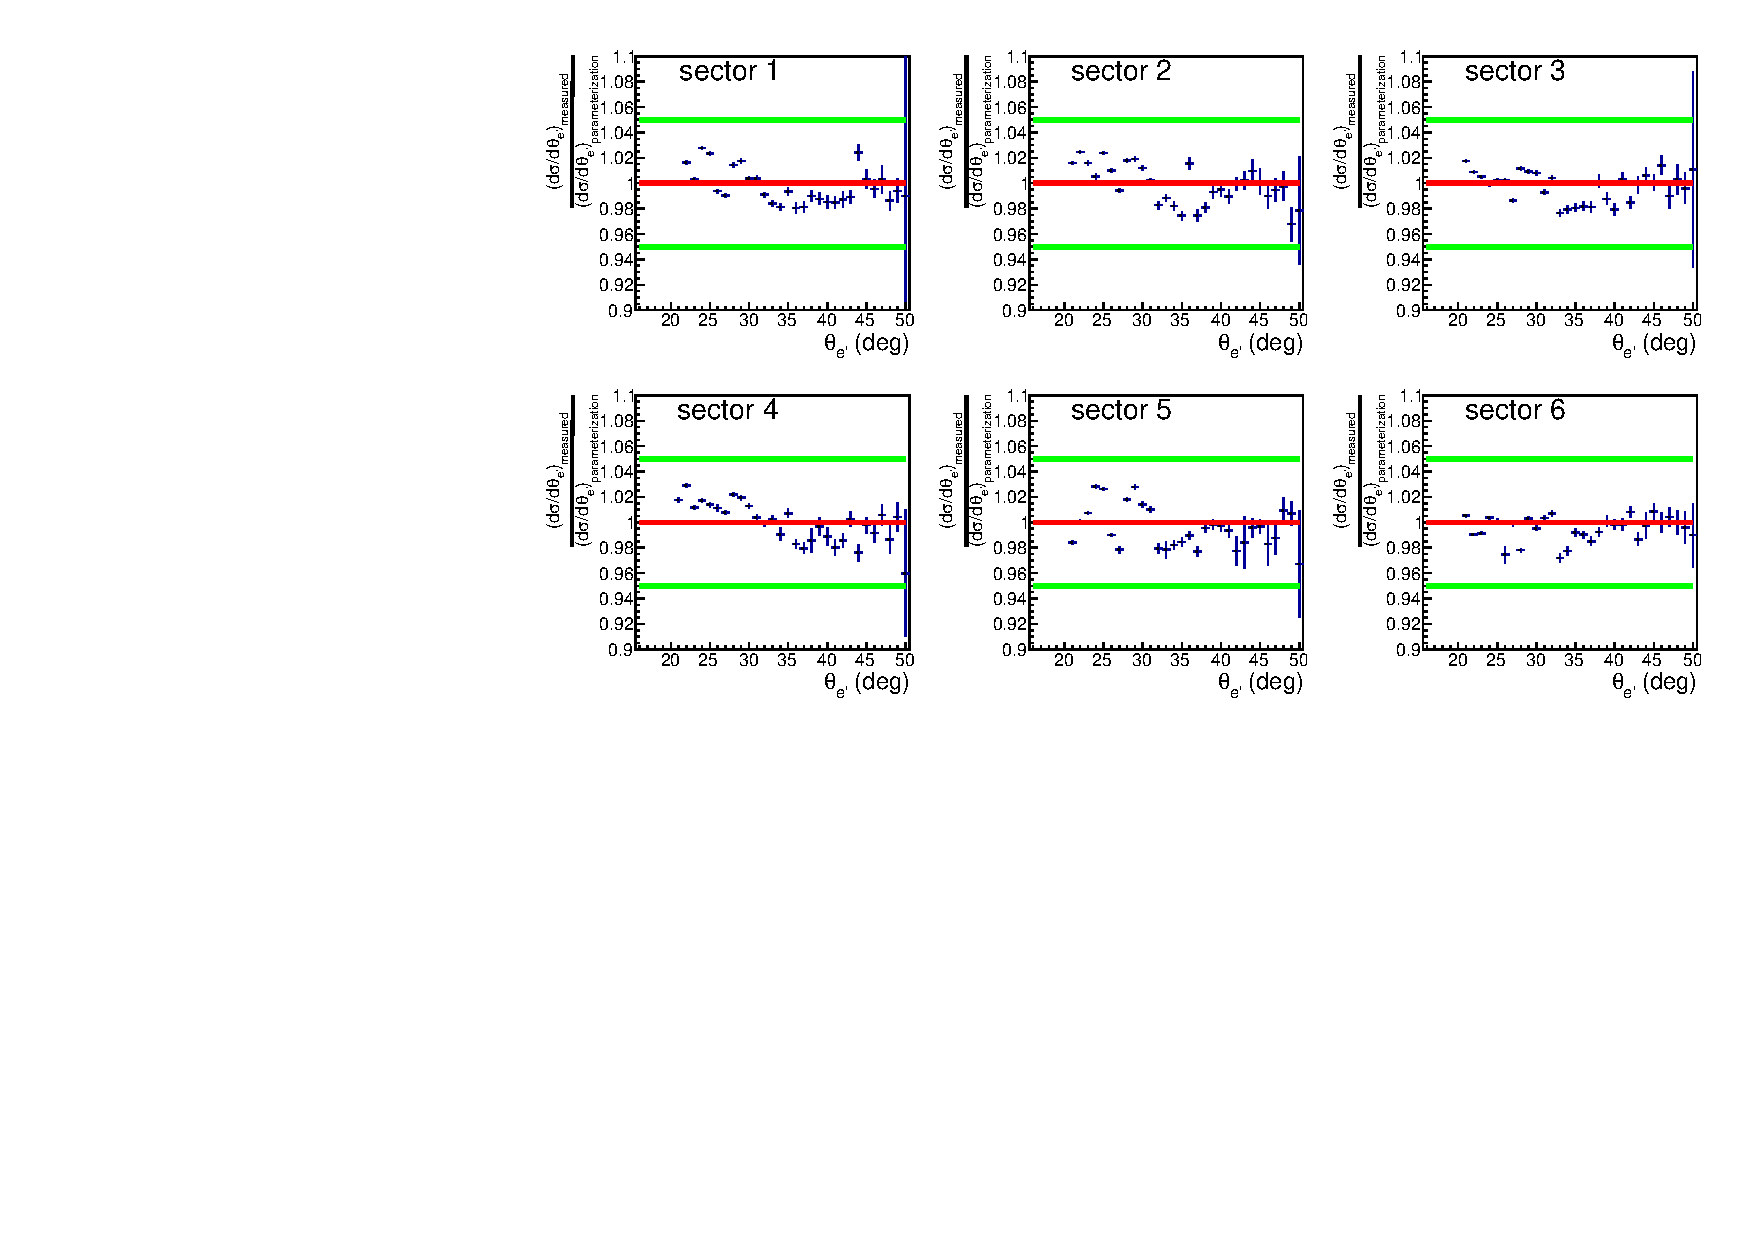
\includegraphics[width=14cm]{pictures/sys_err/elastic/elastic_cross_sect/elast_ratio_6_sectors.pdf}}
\end{center}
\vspace{-0.6cm}
\caption{\small Ratio of the elastic cross
section to the 
parametrization~\cite{Bosted:1994tm},
plotted versus $\theta_{e'}$ angle of the
electron in the lab frame for the six CLAS sectors. Red lines correspond to
unity and green lines indicate a $\pm$5\%
deviation from the parametrization. }
\label{elastcross}
\end{figure}
\newpage

\section{Errors due to the different ways of combining topologies}
\label{var_top_err}

In this analysis two ways of combining topologies are used (see Sect.~\ref{var_top}). The integrated cross sections obtained in these two ways are slightly different. As in the case of the integration over different kinematical grids, this difference is interpreted as systematical error. 
Since different topologies correspond to the different registered final hadrons (and therefore to the different hadron cut combinations) this systematical error includes partially the error due to the shapes of the cuts that are used in the analysis. The error is calculated for each bin in  $W$ and $Q^{2}$ and typically is of the order of 2\%.

\section{Errors due to the integration over different final hadron variables}
\label{integr}

As it is mentioned in Sect.~\ref{kin_var} three sets of kinematical variables are used in this analysis. The cross sections obtained by integration over these three kinematical grids should be the same. However, it is found that they are slightly different due to the fact that data and efficiency propagate differently to the different kinematical grids. This difference is interpreted as systematical error and computed for each bin in $W$ and $Q^{2}$. This systematic effect varies depending on the bin in $W$ and $Q^{2}$ and is typically of the order of 3\%.




\section{Systematical error summary}
\label{syssummary}

\begin{figure}[htp]
\begin{center}
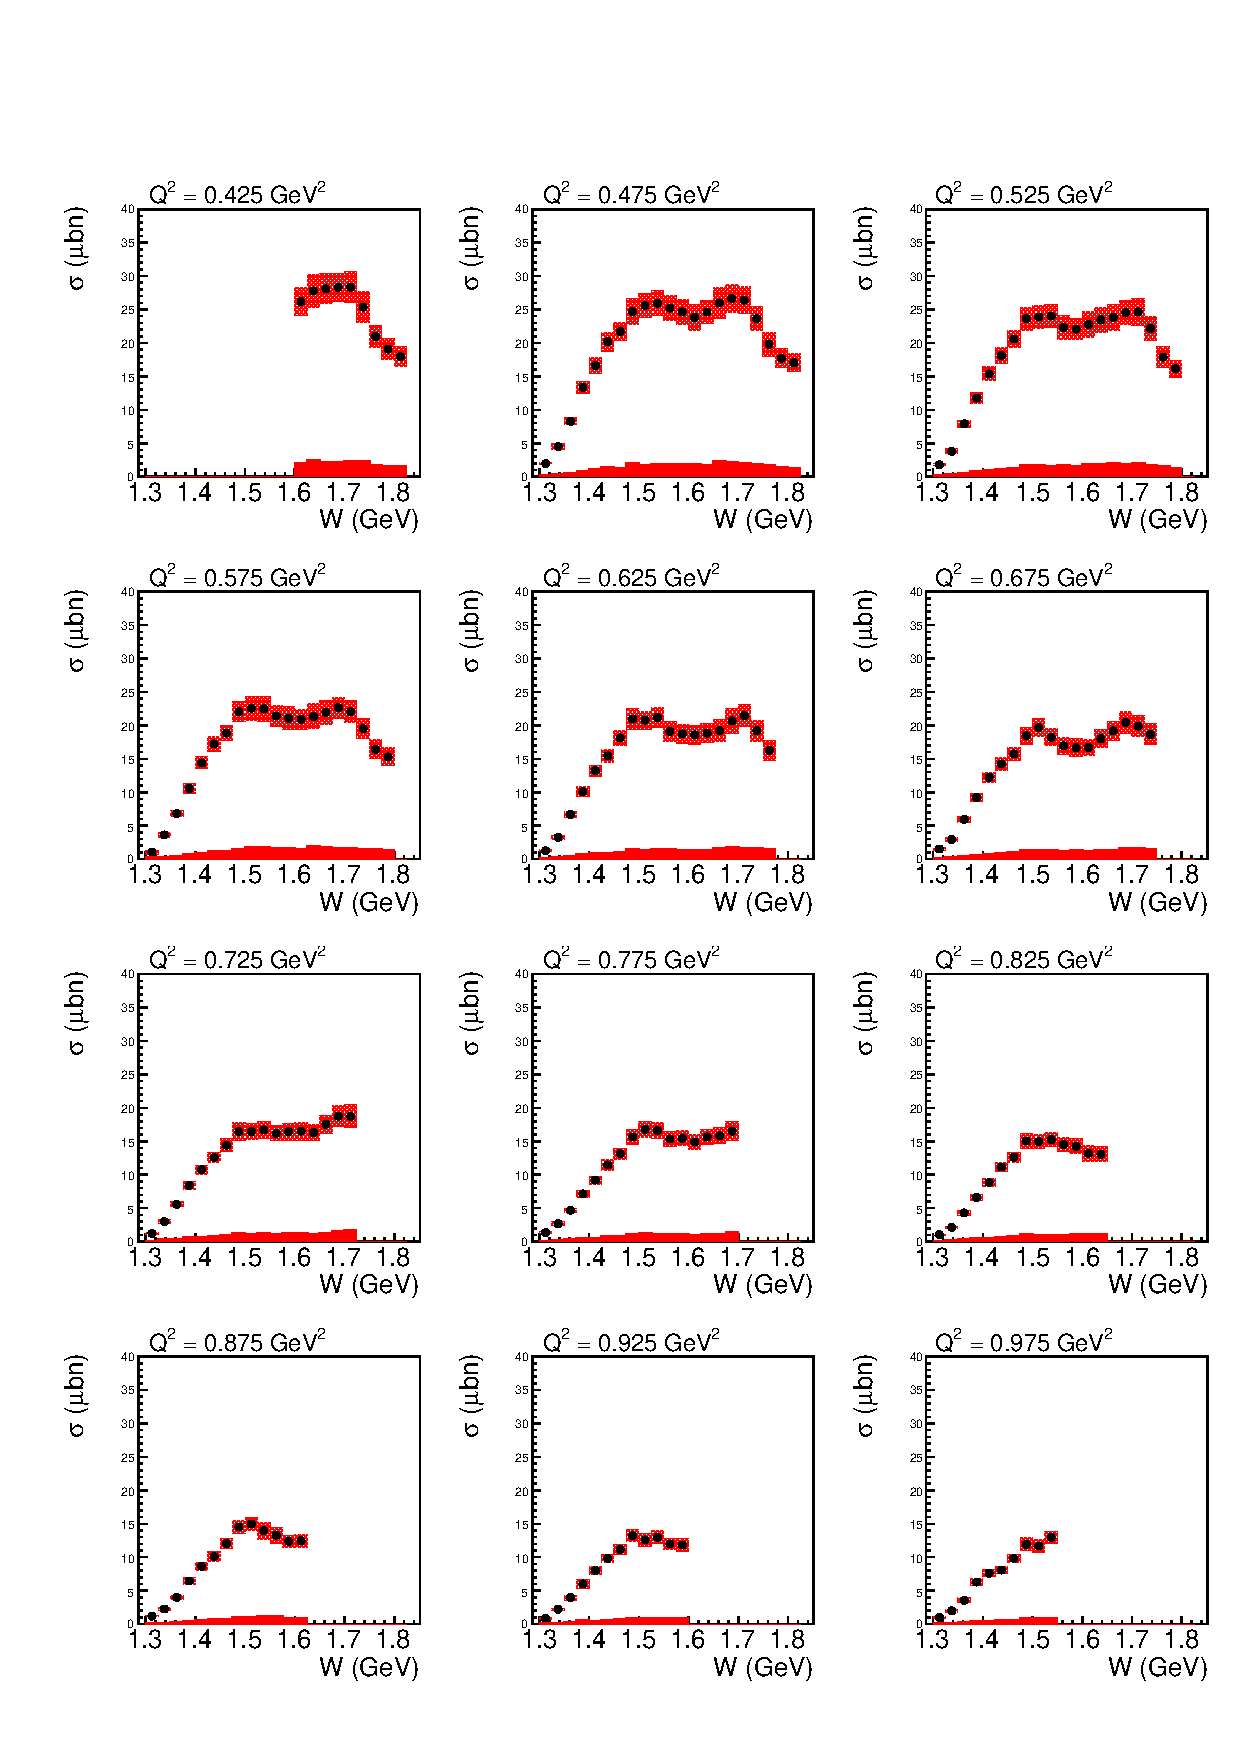
\includegraphics[width=15cm]{pictures/sys_err/sys_err.pdf}
\caption{\small Systematical errors of the integrated cross sections. The plots show $W$ dependencies of the integrated cross section in various bins in $Q^{2}$. The systematical uncertanties are shown as the red bands at the bottom of each plot. The total cross section uncertainty (both statistical and systematical ones summed up in quadrature) is shown by the hatched red areas.}
\label{fig:sys_err}

\end{center}
\end{figure}

As final integrated cross sections, the cross sections that are averaged over three grids of the kinematical variables are reported (see Fig.~\ref{fig:sys_err}). In Fig.~\ref{fig:sys_err} the systematical uncertanties are shown as the red bands at the bottom of each plot. This uncertanties include the errors due to the effects mentioned above and extra 5\% error due to the inclusive radiative corrections procedure (see Sect.~\ref{radiative}). To obtain the red bands all the errors are summed up in quadrature.  

The statistical cross section uncertainties are typically smaller than the systematical ones. The total uncertainty is obtained as the sum of the systematical and statistical ones and is shown by the hatched red areas in Fig.~\ref{fig:sys_err}.
 
The integral systematical errors with their sources are presented in Tab.~\ref{tab:sys_err}.
 
\begin{table}[htp]
\centering 

\begin{tabular}{|c|c|}

\hline
Error source & Error value\\ \hline
Normalization, electron id, and
 electron detection efficiency & 3\% \\ \hline
Different ways of combining topologies & 2\%\\ \hline 
Integration over different final hadron variables & 5\%\\ \hline 
Radiative corrections & 5\% \\ \hline 
\end{tabular}
\caption{\small Systematical error. \label{tab:sys_err}}
\end{table}  

